\documentclass[a4paper]{article}
\usepackage[a4paper, top=1in, left=1.2in, right=1.2in, bottom=1in, footskip=0.25in]{geometry}
\usepackage[absolute]{textpos}
\usepackage{subfigure}
\usepackage{float}
\usepackage{hyperref}
\usepackage{graphicx}
\usepackage{blindtext}
\usepackage{array}
\usepackage{tabularx}
\usepackage{pgfplots}
\pgfplotsset{width=10cm,compat=1.9}
\graphicspath{ {./images/} }
\bibliographystyle{ieeetr}

\title{
	Currying the web: A custom Java 21 REST framework - built on functional paradigms
	- compared to Spring Boot: Ease of Use and Performance
}
\author{Nico Lerchl\\2110257236\\[0.5cm]{\small Advisor: Dipl.-Ing. (FH) Bernhard Wallisch}}

\begin{document}

\begin{textblock}{15}(0.5, 0.5)
	\noindent\Large BACHELOR PAPER\\
	\large Thesis submitted in fulfillment of the requirements for the degree of Bachelor
	of Science in Engineering at the University of Applied Sciences Technikum Wien
	- Degree Program Computer Science\\
\end{textblock}

\maketitle

\newpage

\section*{Declaration}
“As author and creator of this work to hand, I confirm with my signature knowledge of the relevant
copyright regulations governed by higher education acts (see Urheberrechtsgesetz / Austrian
copyright law as amended as well as the Statute on Studies Act Provisions / Examination
Regulations of the UAS Technikum Wien as amended).\newline

\noindent I hereby declare that I completed the present work independently and that any ideas, whether
written by others or by myself, have been fully sourced and referenced. I am aware of any con-
sequences I may face on the part of the degree program director if there should be evidence of
missing autonomy and independence or evidence of any intent to fraudulently achieve a pass
mark for this work (see Statute on Studies Act Provisions / Examination Regulations of the UAS
Technikum Wien as amended).\newline

\noindent I further declare that up to this date I have not published the work to hand nor have I presented
it to another examination board in the same or similar form. I affirm that the version submitted
matches the version in the upload tool.“

\newpage

\section*{Kurzfassung}
\blindtext

\newpage

\section*{Abstract}
\blindtext

\newpage

\section*{Acknowledgements}
\blindtext

\newpage

\tableofcontents

\newpage

\section{Introduction}

Web development is a huge part of the software industry. Most of the time, the server part of a web application
is built using the MVC pattern and object oriented programming \cite{damir2021architecture}.
Functional programming is not used as much in web development, in the last few years however, functional programming
has been gaining a lot of popularity with languages such as Haskell, Scala and Clojure but also with functional concepts
being added to object oriented languages like Java and C\# \cite{klint2022functional}.\newline

\noindent Combining functional programming with web development using more widely used languages e.g. Java is a scarcely
researched topic which this thesis aims to explore and shine some light on. The goal is to build a REST framework
in Java 21 using functional paradigms and compare it to Spring Boot in terms of robustness, error handling and ease of use.

\section{Literature review}
\subsection{REST}

Representational State Transfer (REST) is the state-of-the-art way to build the server part
of a client-server-architecture and it is most likely only going to get bigger in the industry \cite{halili2018web}.
It was first described by Roy Fielding in his doctoral dissertation in 2000.
REST is based on the following properties \cite{fielding2000architectural}:

\begin{itemize}
	\item Client-server - The client and the server are separated and can be developed independently.
	\item Stateless - The server does not store any client state. Every request contains all the information
	      the server needs to process it.
	\item Cache - Responses can be cached to improve performance.
	\item Uniform Interface - The interface between the client and the server is uniform and simple.
\end{itemize}

\subsection{Functional programming}
\subsubsection{General}

Functional programming - unlike procedural or object oriented programming - is not based on the Turing machine,
but rather on lambda calculus. Lambda calculus, developed by Alonzo Church in the 1930s, is a mathematical system
later proven - by Turing himself - to be equivalent to the Turing machine \cite{turing1937computability}.\newline

\noindent The base principles of functional programming are \cite{hughes1989functional}:
\begin{itemize}
	\item Immutability - Variables are not changed after they are assigned a value.
	\item Pure functions - Functions do not have side effects and always return the same output for the same input.
	\item Higher order functions - Functions can be passed as arguments to other functions.
	\item Referential transparency - A function call can be replaced by its return value without changing the program's behavior.
\end{itemize}

\noindent A big part of functional programmings is the concept of monads which have their roots in category theory.
They allow for encapsulating side effects in a pure way. For a container to be a monad
it has to abide by the laws of left identity, right identity and associativity. \cite{wadler1992essence}

\subsubsection{Web development}

Yesod is a web framework for the before mentioned functional programming language Haskell.
It allows developers to build entire websites using templates and widgets or RESTful web services.
Additionally, Yesod offers the ability to persist data using Haskell's type system into
PostgreSQL, SQLite, MySQL, and MongoDB. \cite{snoyman2015developing}

\subsubsection{In Java}

The introduction of lambda expressions in Java 8 brought functional programming to the Java ecosystem.
Where before developers had to use anonymous classes to pass functions as arguments, they can now
use lambda expressions. This also shifts the view point of passing an object that carries functionality
to passing behavior itself. The concept behind these lambda expressions in Java is called functional interfaces.
Functional interfaces are interfaces that have exactly one abstract method. They can be annotated with \verb|@FunctionalInterface|.\newline

\noindent Also new to Java 8 is the Streams API. It hides away the iteration over collections by offering
many higher order functions. Additionally, streams are only evaluated when a terminal operation, such as
collecting, counting or averaging is called, implementing the - before mentioned -
functional programming principle of lazy evaluation. \cite{warburton2014java}

\subsection{Spring Boot}

Spring Boot is a framework for building stand-alone web applications and RESTful web services in Java.
Unlike Spring Framework there is zero requirement for XML configuration. It can be deployed using an internal web server
or going the classic route of deploying a war file onto an external web server. \cite{webb2013spring}

\section{Research questions and hypotheses}
\subsection{Research questions}

All of the following questions will be answered by comparing the custom framework to Spring Boot.

\begin{enumerate}
	\item Will building a web application using functional paradigms naturally guide the developer to
	      eliminate unwanted behavior?
	\item Will the developer experience benefit from developing a REST API using
	      functional paradigms from the ground up?
\end{enumerate}

\subsection{Hypotheses}

\begin{enumerate}
	\item Building a web application using functional paradigms will naturally guide the developer to
	      eliminate unwanted behavior. Common pitfalls of object oriented programming such as mutable state,
	      side effects, null references and unchecked exceptions will be avoided. Null values are practically omitted
	      and exceptions handled gracefully through the use of monads.
	\item The developer experience will benefit as error handling becomes more natural and testing becomes less
	      of a burden because functions will always produce the same output for the same input and not rely
	      on external factors. Additionally, the declarative nature of functional programming
	      will increase conciseness and expressiveness directly leading to less
	      lines required to achieve similar results.
\end{enumerate}

\section{Methodology}
ChatGPT 4 was prompted to generate a simple REST API for a todo list application
using Curryful and Spring Boot. The prompts are identical besides having to
provide more information about Curryful, as ChatGPT does not know about this new
framework. The prompts and any changes that had to be done to the generated code
are available in the projects' repositories
(\hyperlink{https://github.com/lerchl/curryful-bachelor-thesis-curryful-todo-list-preview-features}{Curryful
	- using Java 21's preview features},
\hyperlink{https://github.com/lerchl/curryful-bachelor-thesis-curryful-todo-list}{Curryful} and
\hyperlink{https://github.com/lerchl/curryful-bachelor-thesis-spring-boot-todo-list}{Spring Boot}).

\subsection{Provoking unwanted behavior using invalid requests}
The prompts were held short and do not explicitly ask for any implementation details except for using in-memory storage
and for the Curryful project to parse JSON using \hyperlink{https://github.com/FasterXML/jackson}{Jackson}.\newline

\noindent Using Postman, both application generated by ChatGTP were sent requests trying to provoke
unwanted behavior. The applications were restarted after each request to assure
no side effects could mess with the results. The requests can be found in the
form of JSON, exported by Postman as a collection v2.1
\hyperlink{https://github.com/lerchl/curryful-bachelor-thesis-postman-requests}{here}.\newline

\noindent The requests are:
\begin{itemize}
	\item POST request where "completed" is a string
	\item POST request where a car is added
	\item POST request where the body is empty
	\item GET request for id -1
	\item PUT request for id -1
	\item POST request to toggle completed for id -1
	\item DELETE request for id -1
	\item GET request for id test
	\item GET request for id 999999999999999999999
\end{itemize}

\subsection{Static code analysis}
The generated code was analyzed using SonarCloud to determine both cyclomatic
and cognitive complexity. The cyclomatic complexity is a measure of the number
of linearly independent paths through a program's source code and therefore also
represents the number of test cases required to reach a coverage of 100\%.
Cognitive complexity describes how hard it is for a person to understand the
code. Sonar was not able to analyze the Curryful project using Java 21's preview
features of unnamed classes and instance main methods, hence the need for two
Curryful repositories.
Kann ich das einfach so sagen?
Brauch ich hier eine Quelle für? Kann ich irgendwie sagen, dass Sonar das halt so beschreibt? \newline

\noindent An additional measure to determine developer experience is the number
of lines of code. Sonar would also provide this metric, since using Java 21's
review features of unnamed classes and instance main methods are a part of this
thesis however, lines of code were counted manually following these rules:

\begin{itemize}
	\item empty lines are not counted
	\item package declarations are not counted
	\item imports are not counted
	\item comments are not counted
	\item lines must not be longer than 120 characters
	\item each added part of a method chain should be in a new line, unless
	      the entire chain is not longer than 120 characters
\end{itemize}

\newpage

\section{Results}
\subsection{Provoking unwanted behavior using invalid requests}
\begin{table}[h!]
	\begin{tabularx}{\textwidth}{|X|c|c|c|}
		\hline
		\textbf{Request}                           & Expected status code & \multicolumn{2}{c|}{Actual status code}               \\
		                                           &                      & Curryful                                & Spring Boot \\
		\hline
		POST request where "completed" is a string & 400                  & 400                                     & 400         \\
		POST request where a car is added          & 400                  & 400                                     & 200         \\
		POST request where the body is empty       & 400                  & 400                                     & 400         \\
		GET request for id -1                      & 404                  & 404                                     & 200         \\
		PUT request for id -1                      & 404                  & 404                                     & 200         \\
		POST request to toggle completed for id -1 & 404                  & 404                                     & 200         \\
		DELETE request for id -1                   & 404                  & 404                                     & 200         \\
		GET request for id test                    & 400                  & -                                       & 400         \\
		GET request for id 999999999999999999999   & 400                  & -                                       & 400         \\
		\hline
	\end{tabularx}
	\caption{Results of the invalid requests}
\end{table}

\noindent The project using Curryful responded with the expected status code
seven out of nine times. The two times it did not respond with the expected
status code, the application crashed and did not respond at all. This is an
oversight by ChatGTP which tried parsing the id path parameter to an integer,
without checking if it is actually an integer:

\begin{verbatim}
	context.getPathParameters().get("id").map(Integer::parseInt)
\end{verbatim}

\noindent More than just an oversight by ChatGPT, this is a massive error in the
Curryful framework itself.
\newline

\noindent The project using Spring Boot responded with the expected status code
four out of nine times. The POST request adding a car created a todo without a
title. All requests trying to access a non-existent todo with the id -1,
returned 200, making it seem like the todo actually exists.

\subsection{Static code analysis}
\begin{center}
	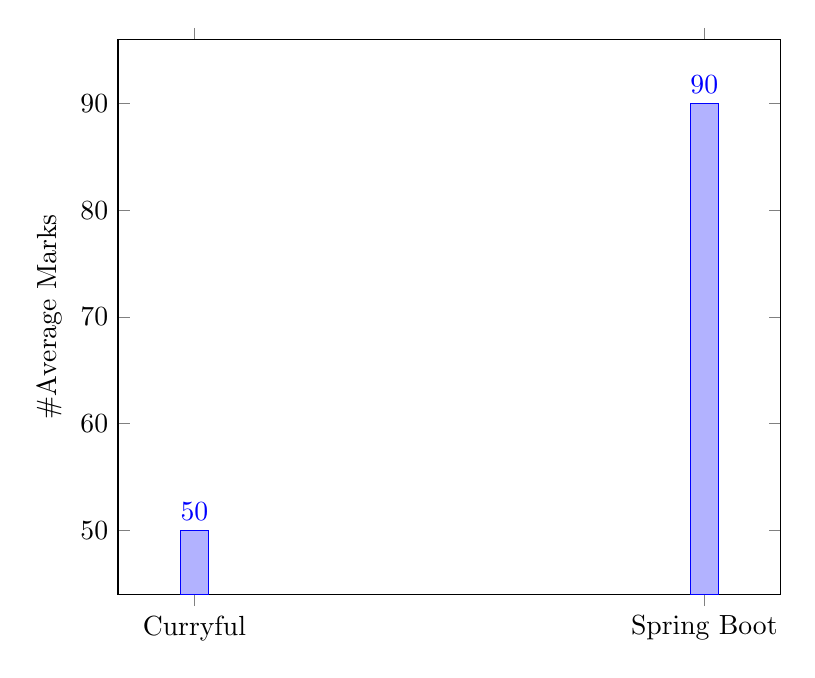
\begin{tikzpicture}
		\begin{axis}
			[
				ybar,
				enlargelimits=0.15,
				ylabel={\#Average Marks}, % the ylabel must precede a # symbol.  
				symbolic x coords={Curryful, Spring Boot}, % these are the specification of coordinates on the x-axis.  
				xtick=data,
				nodes near coords, % this command is used to mention the y-axis points on the top of the particular bar.  
				nodes near coords align={vertical},
			]
			\addplot coordinates {(Curryful,50) (Spring Boot,90)};
		\end{axis}
	\end{tikzpicture}

	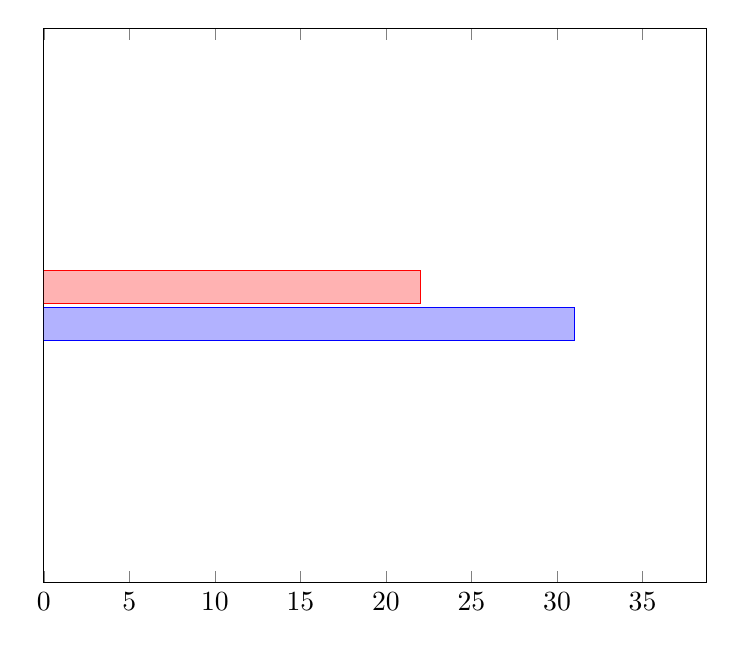
\begin{tikzpicture}
		\begin{axis} [
				xbar = .05cm,
				bar width = 12pt,
				xmin = 0,
				enlarge y limits = {abs = .8},
				enlarge x limits = {value = .25, upper},
				ytick
			]
			\addplot coordinates {(31,0)};
			\addplot coordinates {(22,0)};

		\end{axis}
	\end{tikzpicture}

	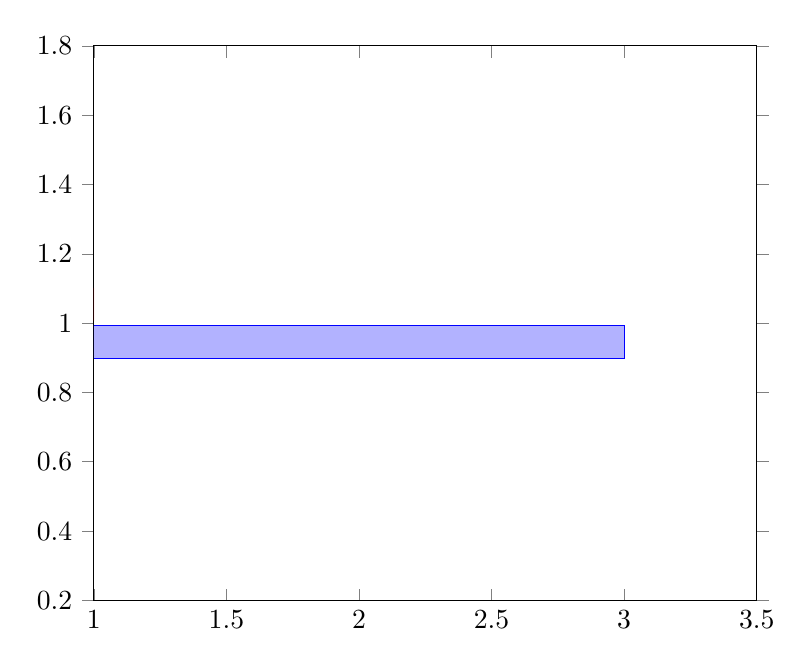
\begin{tikzpicture}
		\begin{axis} [
				xbar = .05cm,
				bar width = 12pt,
				enlarge y limits = {abs = .8},
				enlarge x limits = {value = .25, upper},
			]
			\addplot coordinates {(3,1)};
			\addplot coordinates {(1,1)};

		\end{axis}
	\end{tikzpicture}

	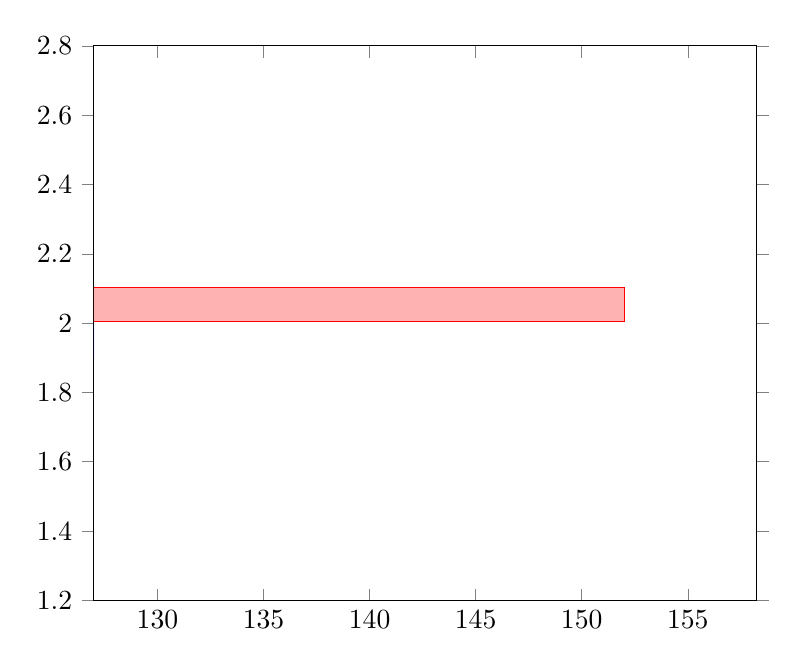
\begin{tikzpicture}
		\begin{axis} [
				xbar = .05cm,
				bar width = 12pt,
				enlarge y limits = {abs = .8},
				enlarge x limits = {value = .25, upper},
			]
			\addplot coordinates {(127,2)};
			\addplot coordinates {(152,2)};

		\end{axis}
	\end{tikzpicture}
\end{center}
\newpage

\listoffigures
\newpage

\listoftables
\newpage

\bibliography{ref}

\end{document}
